Initially, the raw data in the .csv files was distributed in multiple files (one file per user, per time interval). The files were read in and processed by the Python Pandas\footnote{\url{https://pandas.pydata.org}} tool. The library offers fast and flexible functionalities for data analysis. It utilises DataFrames which are fast and efficient 2D data structures, used to store tabular data. Using the Pandas read\_csv and concat methods, the files with identical time periods were transformed and concatenated to one collective DataFrame. 


\subsubsection{Missing Values}
The raw data contained several rows with empty cells. Section \ref{section:MissingValues} lists approaches on how to substitute missing data, thus preserving the row, which could otherwise contain important information. In doing so however, the existing patterns could be disrupted. In order maintain the data's patterns, rows with missing values were removed. Using the Pandas' dropna\footnote{\url{https://pandas.pydata.org/pandas-docs/stable/reference/api/pandas.DataFrame.dropna.html}} function (deletes rows with missing values), all rows containing empty cells were dropped. Of the original 8283 rows from the 1 hour time period files, only 3279 (39.59\%) rows were complete and remained. In the 3 hour files, only 6218 from 14091 (44.13\%) persisted.

\subsubsection{Normalisation}
The data recorded from the different smartphone sensors returned values with different ranges. For example, whilst the values that describe the screen on time ranged between -20 and 2.0, the light sensor values could reach from 0 to over 60,000. As explained in \ref{section:Normalisation}, values with higher ranges can inadvertently outweigh smaller values. To be sure that the values are weighted the same, \textit{Min-Max Normalization} was used to map all the values into the common range, e.g. [0,1]. The sklearn MinMaxScaler was initially used to calculate the new, normalised values in the data set. Most of the values in the data set ranged between 0 and just over 100. The light sensor values were the exception, with its values reaching above 60,000. As mentioned in section \ref{section:Normalisation}, Z-score normalization is more robust to outliers, that could otherwise bias Min-Max Normalization. Therefore, the sklearn StandardScaler was used instead of the MinMaxScaler, which implements the Z-score normalization.

\subsubsection{Selection of columns (attributes)}
% TODO:
% Also - compressing 1-N columns
In order to only use meaningful data to receive significant results, it was important to remove columns that do not contain any predictive content. The TIME column was removed for this reason. Since the TIME column only showed the time and data when the data was recorded periodically (in fixed intervals), it was \textbf{serial ???????} data that had no influence on the data or any predictive value (like an index). It could have however bias the results if left in. 

To reduce the number of dimensions (number of columns), columns with the same feature (e.g. ACC1-N) were compressed to one column. Each unique feature only requires one column, and therefore reduced the number of columns to only 8 (instead of 32 in the 1h data set or 48 in the 3h data set).


\subsubsection{Chain shaped data}
Initial visualisations of the data set (with t-SNE dimensionality reduction) showed a chain formalisation of the data. This chain can be seen in figure \ref{figure:tsneChain} (light blue data points). A similar accumulation of data points, though this time shaped as a line, can further also be seen in the PCA dimensionality reduced data set (see figure \ref{figure:pcaChain}). 


\begin{figure*}[h]
  \centering
  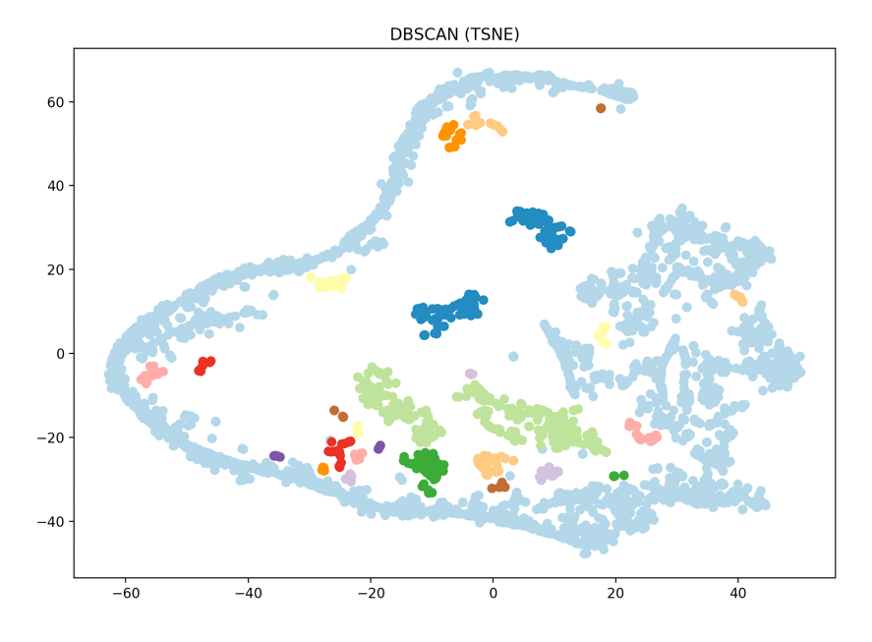
\includegraphics[width=1\textwidth]{./images/tsneChain.png}
  \caption{1h data set, a chain of data points (light blue points) can be seen in the data set.}
  \label{figure:tsneChain}
\end{figure*}


\begin{figure*}[h]
  \centering
  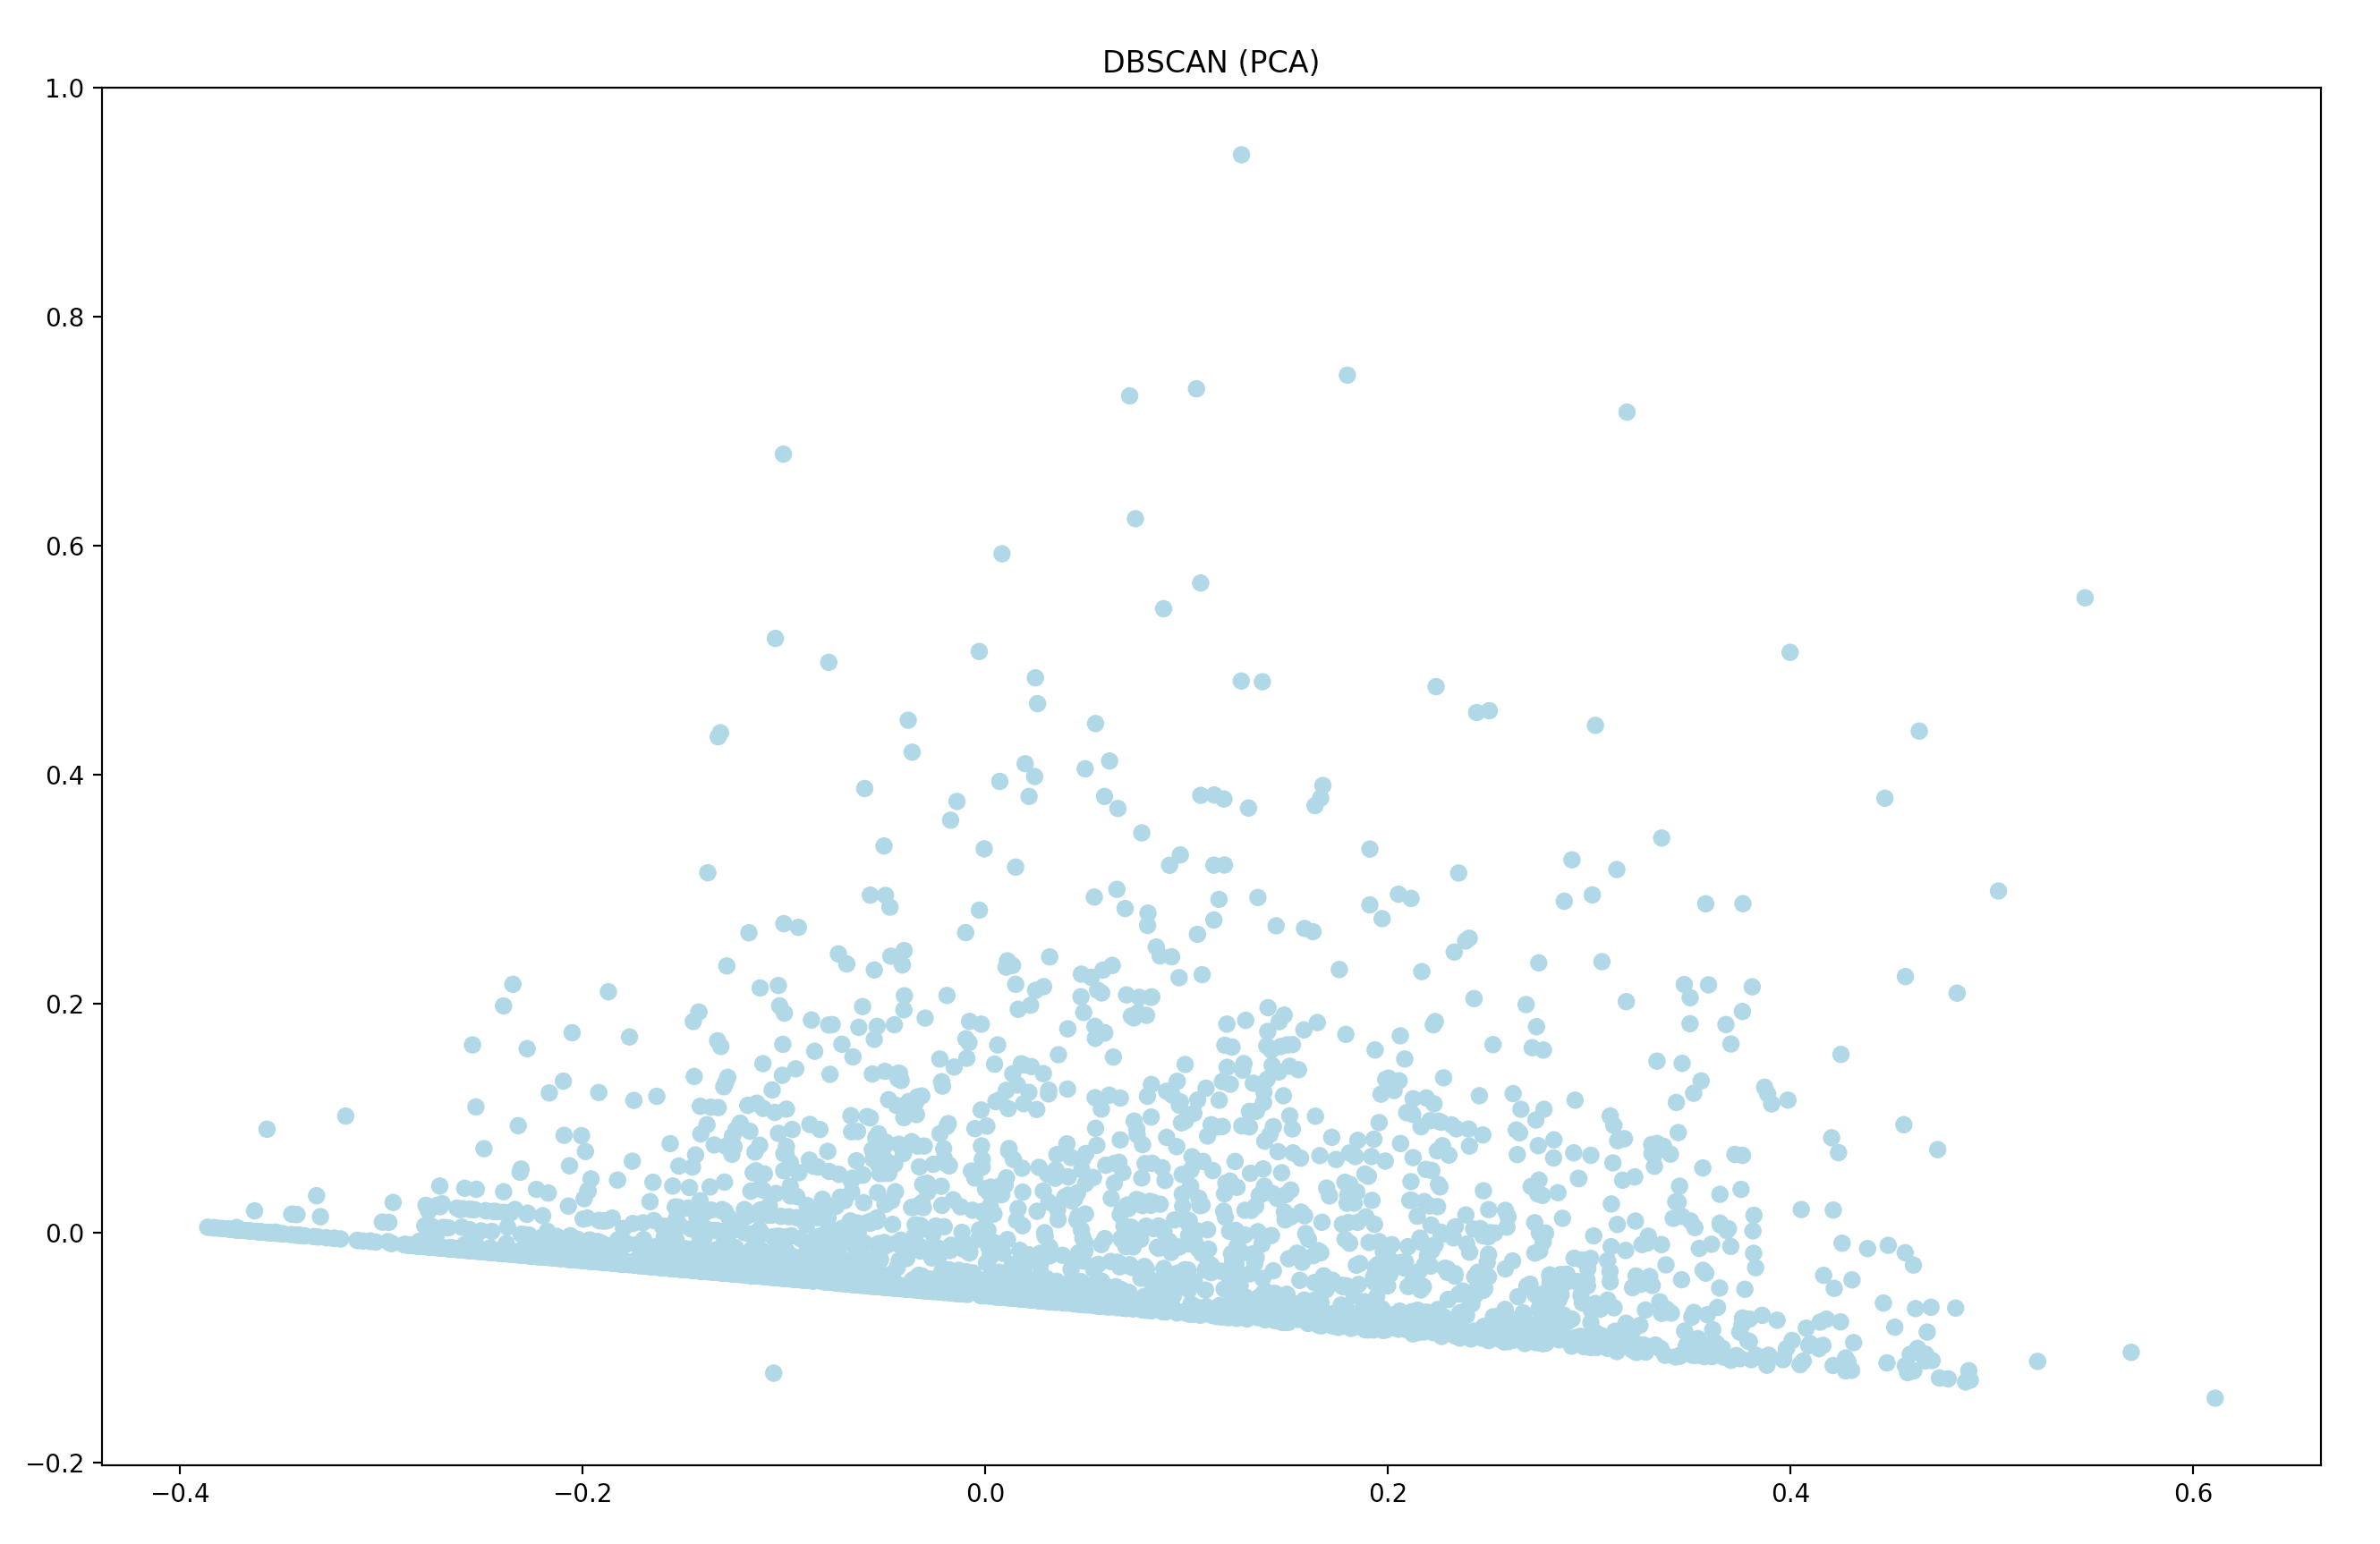
\includegraphics[width=1\textwidth]{./images/pcaChain.png}
  \caption{There is a collection of points along a line. This same collection can also be visualised as a chain in the t-SNE data set.}
  \label{figure:pcaChain}
\end{figure*}

An initial thought, was that this chain was the result of the utilised t-SNE parameters. However, even with changing the t-SNE perplexity, learning rate and number of iterations parameters, the chain persisted in some form. Another thought, as to where these data points originated from or why they resulted in a chain, was that there were dependencies within the data or columns. For example the three APP columns, these indicate the percentage of time in a lag-interval that a type of app was used. Therefore, if say a communication app was used 100\% of this time, the APP\_COM cell for this time would be 1. By using this app for 100\% of the time, would mean that the values in the other APP columns for this time would have to be 0 (0\%), since they would not have been able to be used. To test this theory, the APP columns were removed from the data set and the 2D scatter plot was recalculated. The chain was still visible. Step by step each column was removed, to see if it was the cause of the chain. The chain did not disappear though, which indicated, that the problem was not due to the columns, but rather the rows. The chain was less visible when reducing the number of inserted .csv files (lower number of records) to 10 (see figure \ref{figure:tsne10Files}). When the number of features were reduced to only AUDIO and ACC (two columns), the chain was once again visible (see figure \ref{figure:tsne10Files2Features}). The presumption is that when there are less data points and more features (e.g. 10 files but using all the features), there are enough different data points and the chain less dense, making it less noticeable. When there are less data points but with less features (e.g. 10 files but using only 2 features), or when there are many data points even with multiple features (e.g. all data files and all the features), there are more rows with very similar of equal values and the chain appears more dense and prevalent.

\begin{figure*}[h]
  \centering
  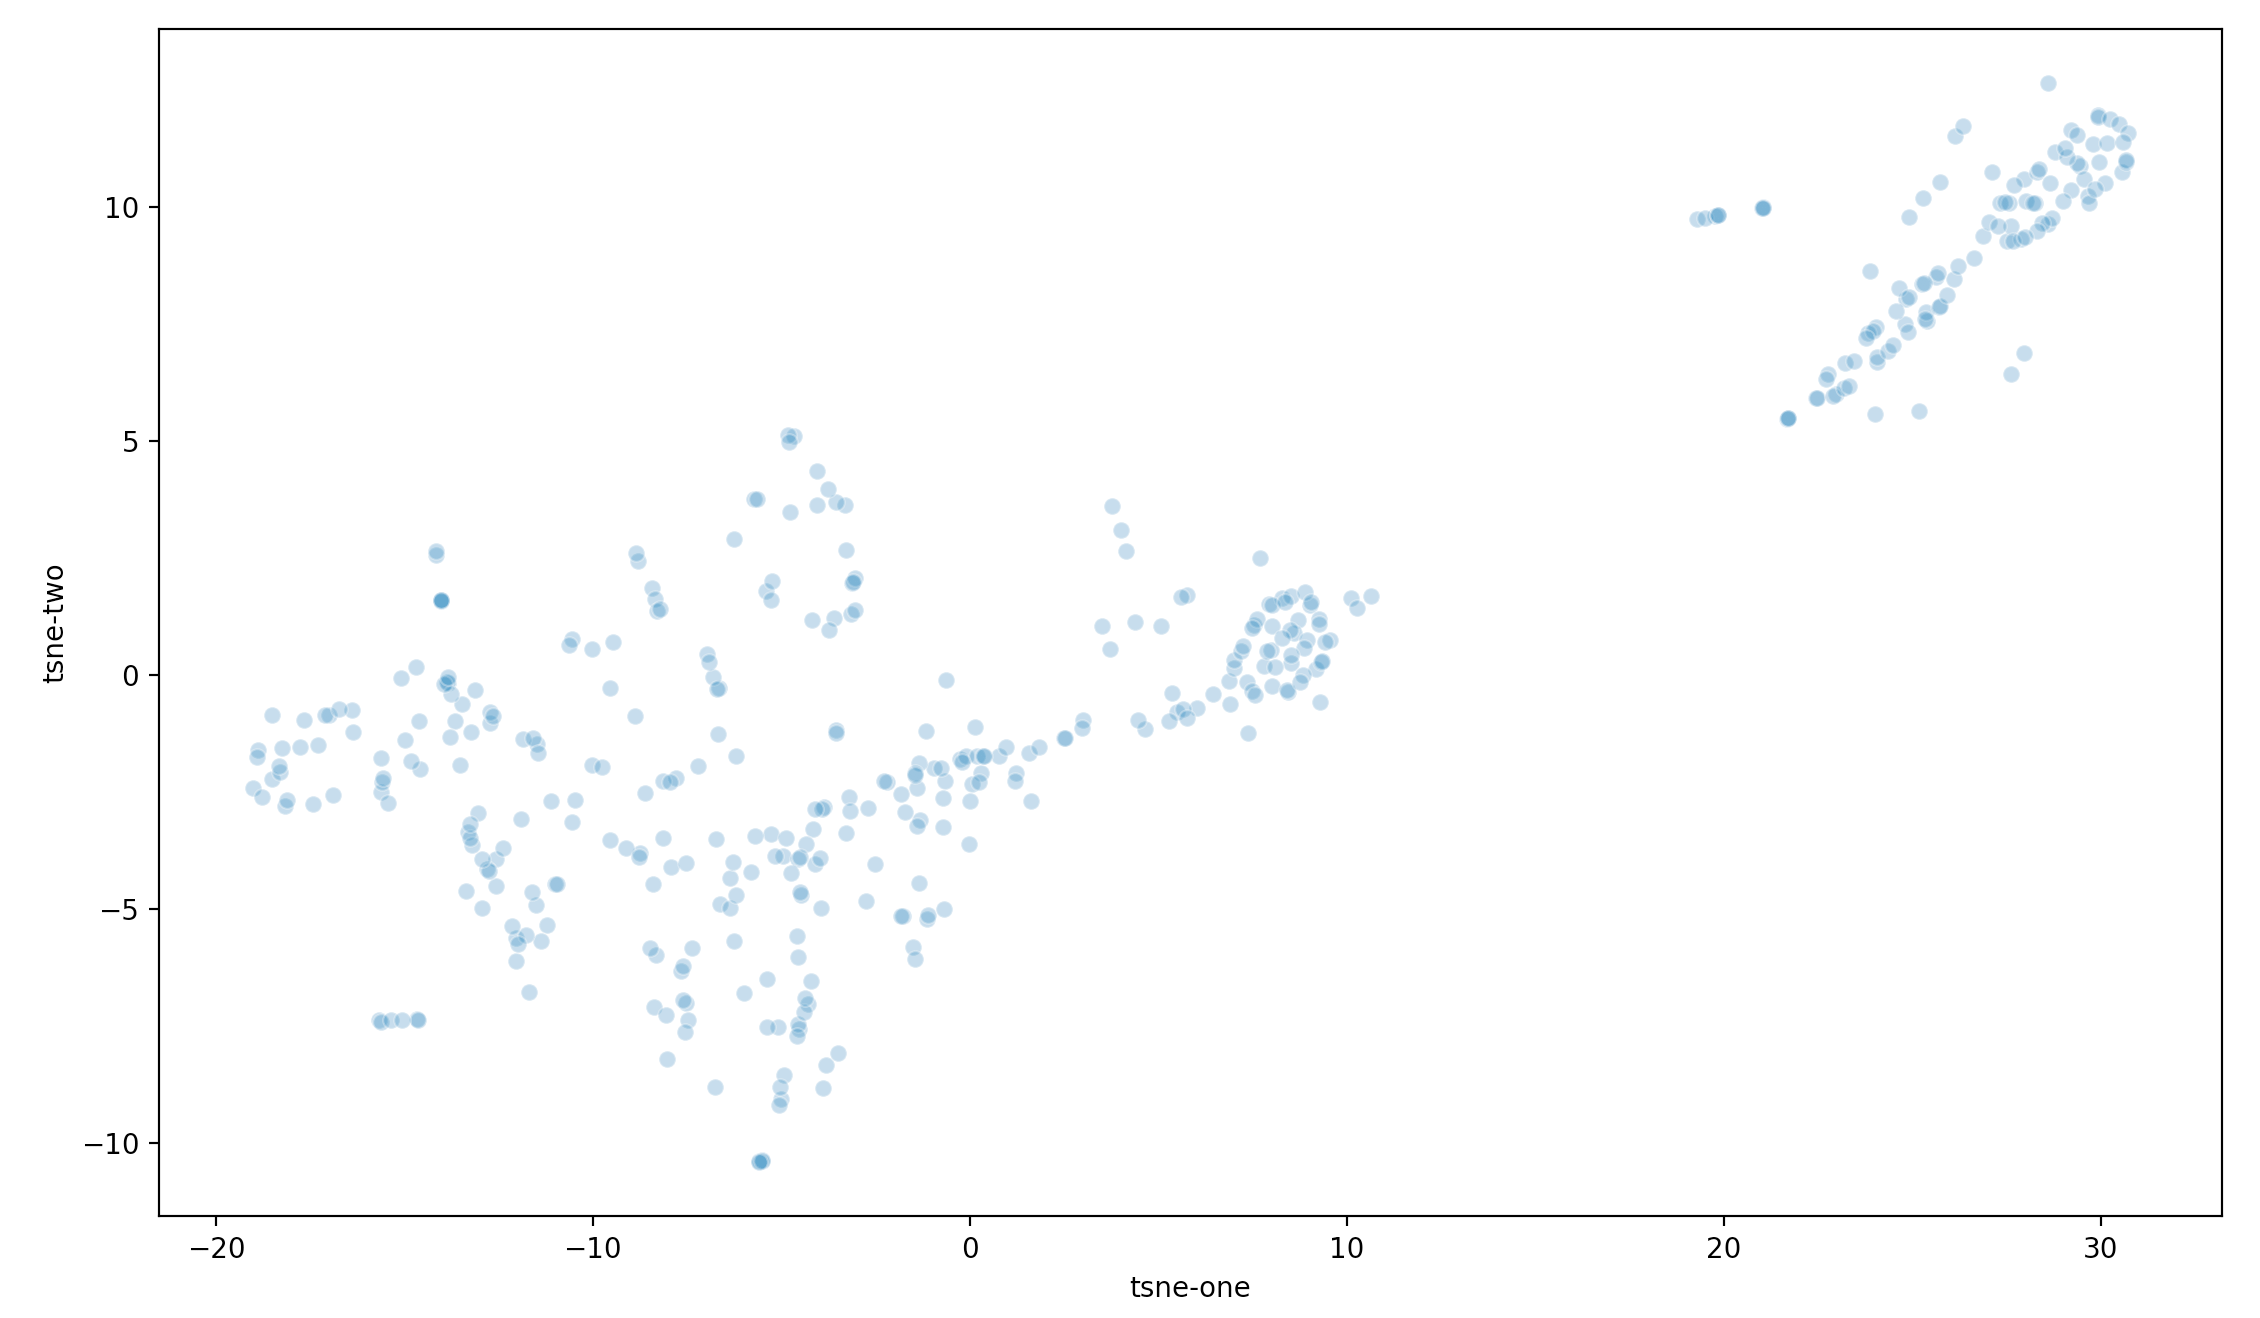
\includegraphics[width=0.5\textwidth]{./images/tsne10Files.png}
  \caption{t-SNE calculated with only 10 data files and all features. The chain is as visible.}
  \label{figure:tsne10Files}
\end{figure*}

\begin{figure*}[h]
  \centering
  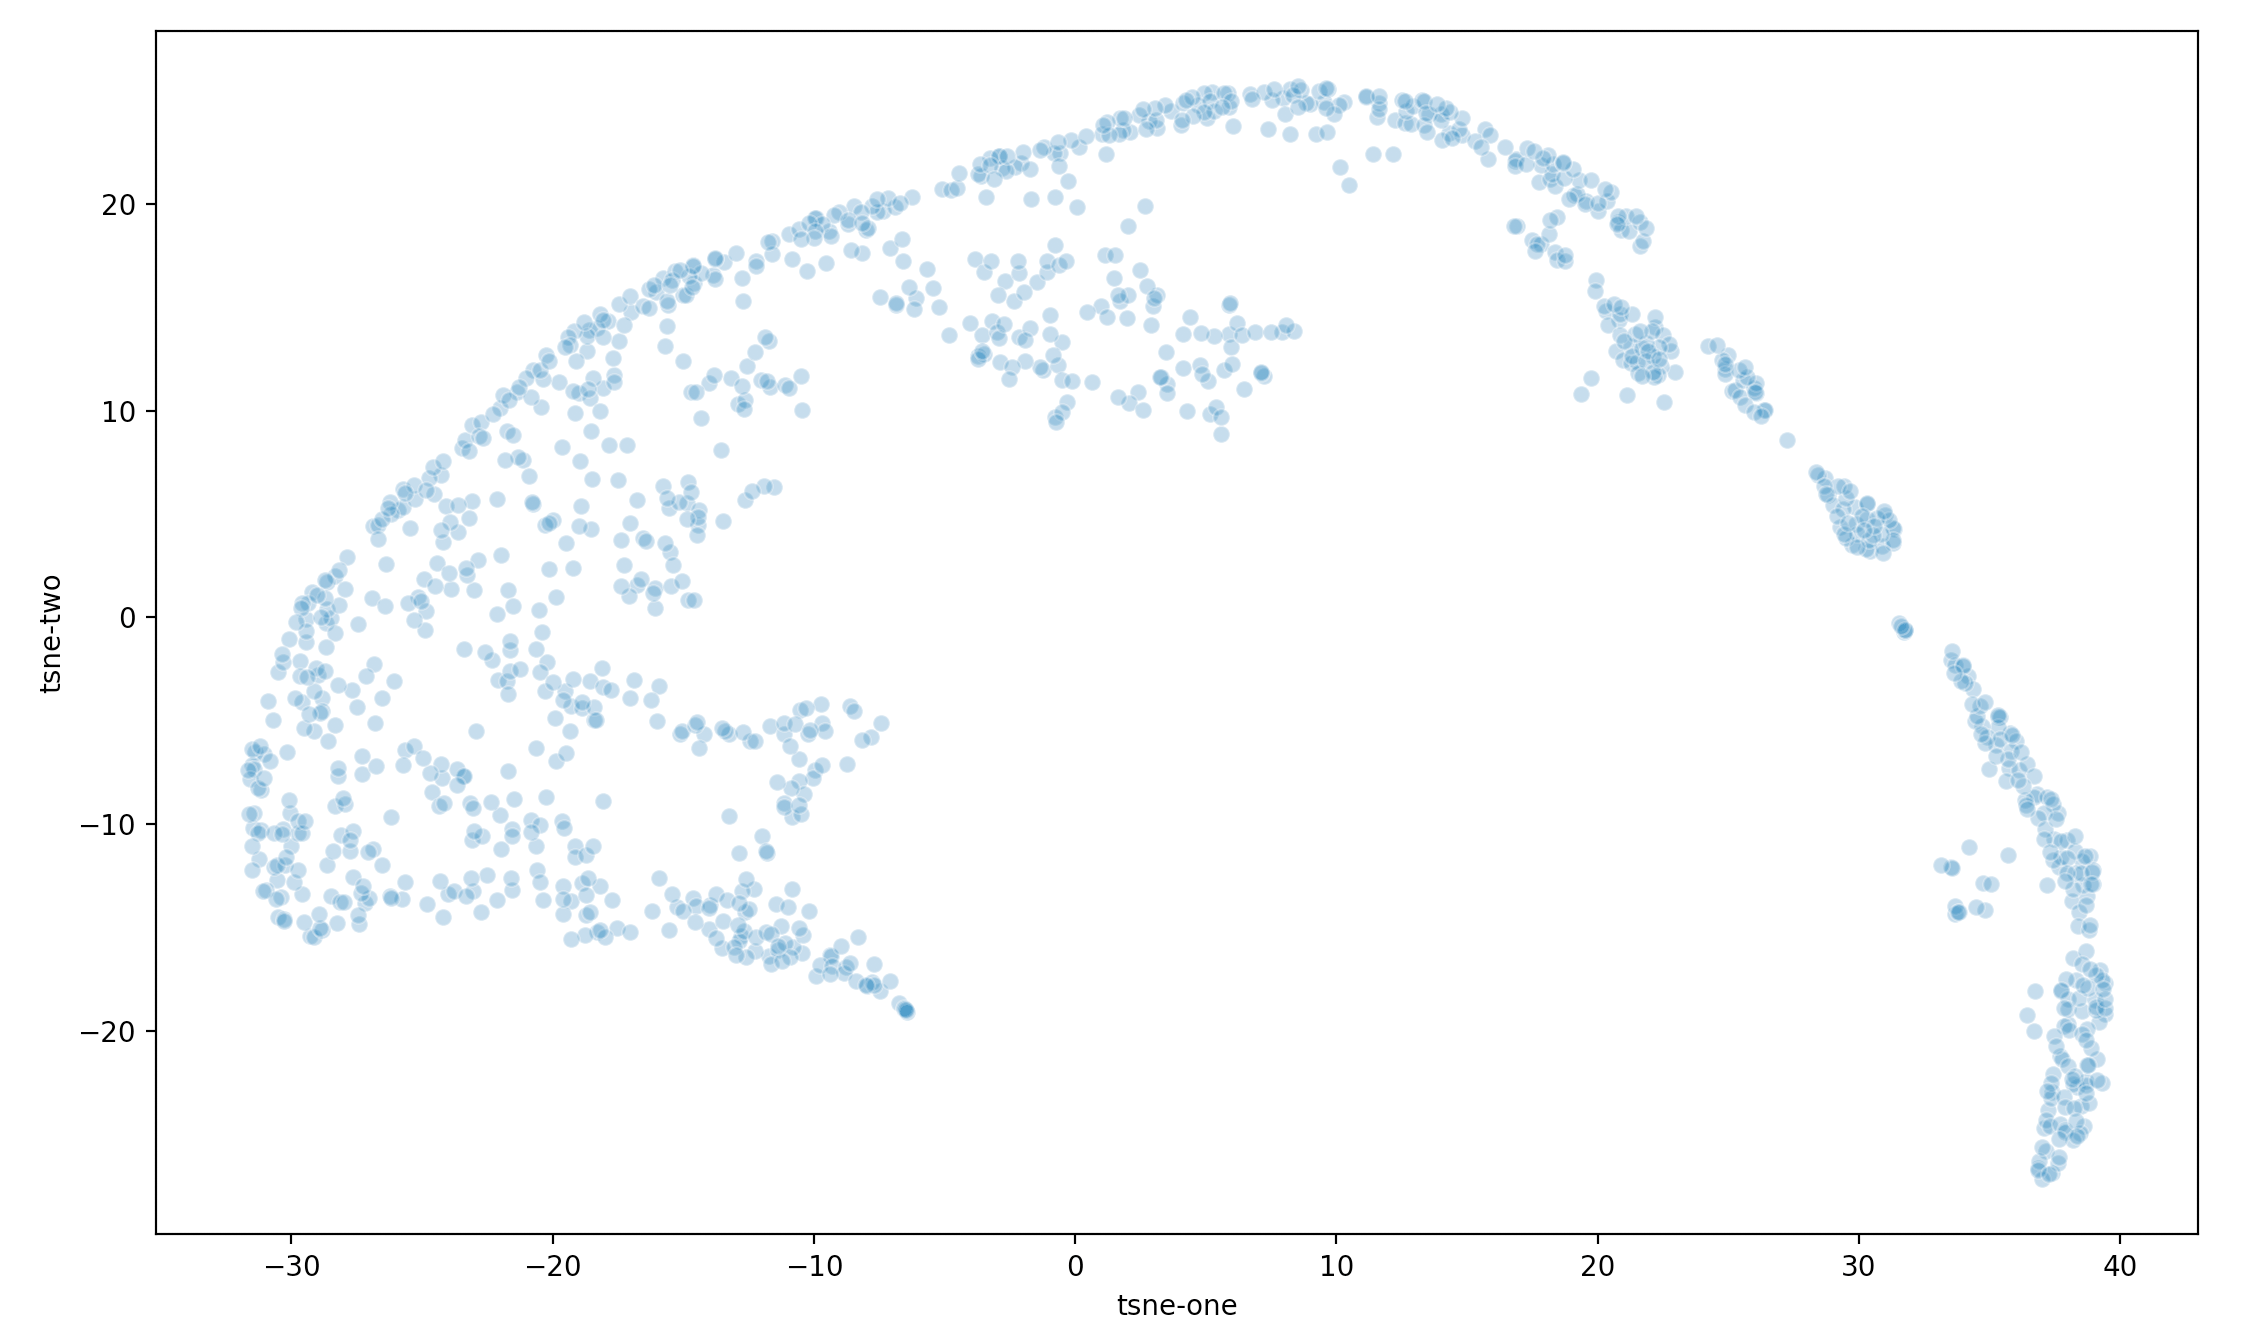
\includegraphics[width=0.5\textwidth]{./images/tsne10Files2Features.png}
  \caption{t-SNE calculated with 10 data files and only 2 features. The chain is visible.}
  \label{figure:tsne10Files2Features}
\end{figure*}

One theory was that points from a same test subject were similar and might be causing the chain. To see which data points were contained in the chain, the row index number was added as a label to each data point in the scatter plot. Furthermore, each test user data file was assigned a different random colour, so that in the plot it was visible, which data points belonged to the same user. The resulting scatter plot is visualised in figure \ref{figure:tsneTestSubjectsColor}. From this plot it can be seen, that several data points from the same test subject cluster together in the chain, indicating similarity. There are however points from each user in different locations of the chart, not only in the chain. This implied, that the chain was not being caused by the subjects. 

The next step was to use the data point indices and to look for similarities in the values. Several rows found in the chain were extracted from the cleaned data set, directly before being fed into the t-SNE algorithm. After comparing these, it was evident that they shared a lot of the same feature values. Rows not in the chain however had different values. Looking at the same rows in the uncleaned data set (after concatenation of the .csv data files and removal of rows with missing values), rows found in the chain had several columns all with the value 0. Further inspection showed, that when the SCRN value was 0, LIGHT, NOTIF and the APP columns where also 0. When a smartphone screen is off, the apps are not being used, which explains why the APP columns were mostly 0. The NOTIF values were often 0, presumably because the user was not constantly receiving notifications. The environment light is also often 0 when a phone is not being used, maybe because it is in a pocket or bag. To test whether these rows were causing the chain to occur, rows with less than 50\% of values that weren't 0 were removed. As can be seen in figure \ref{figure:tsneAfterChainRemoved(50Percent)} \textbf{TODO: ADD FIGURE FROM LATEST}, the chain is only slightly visible. The colours belonging to the test users are also more distributed.


\begin{figure*}[h]
  \centering
  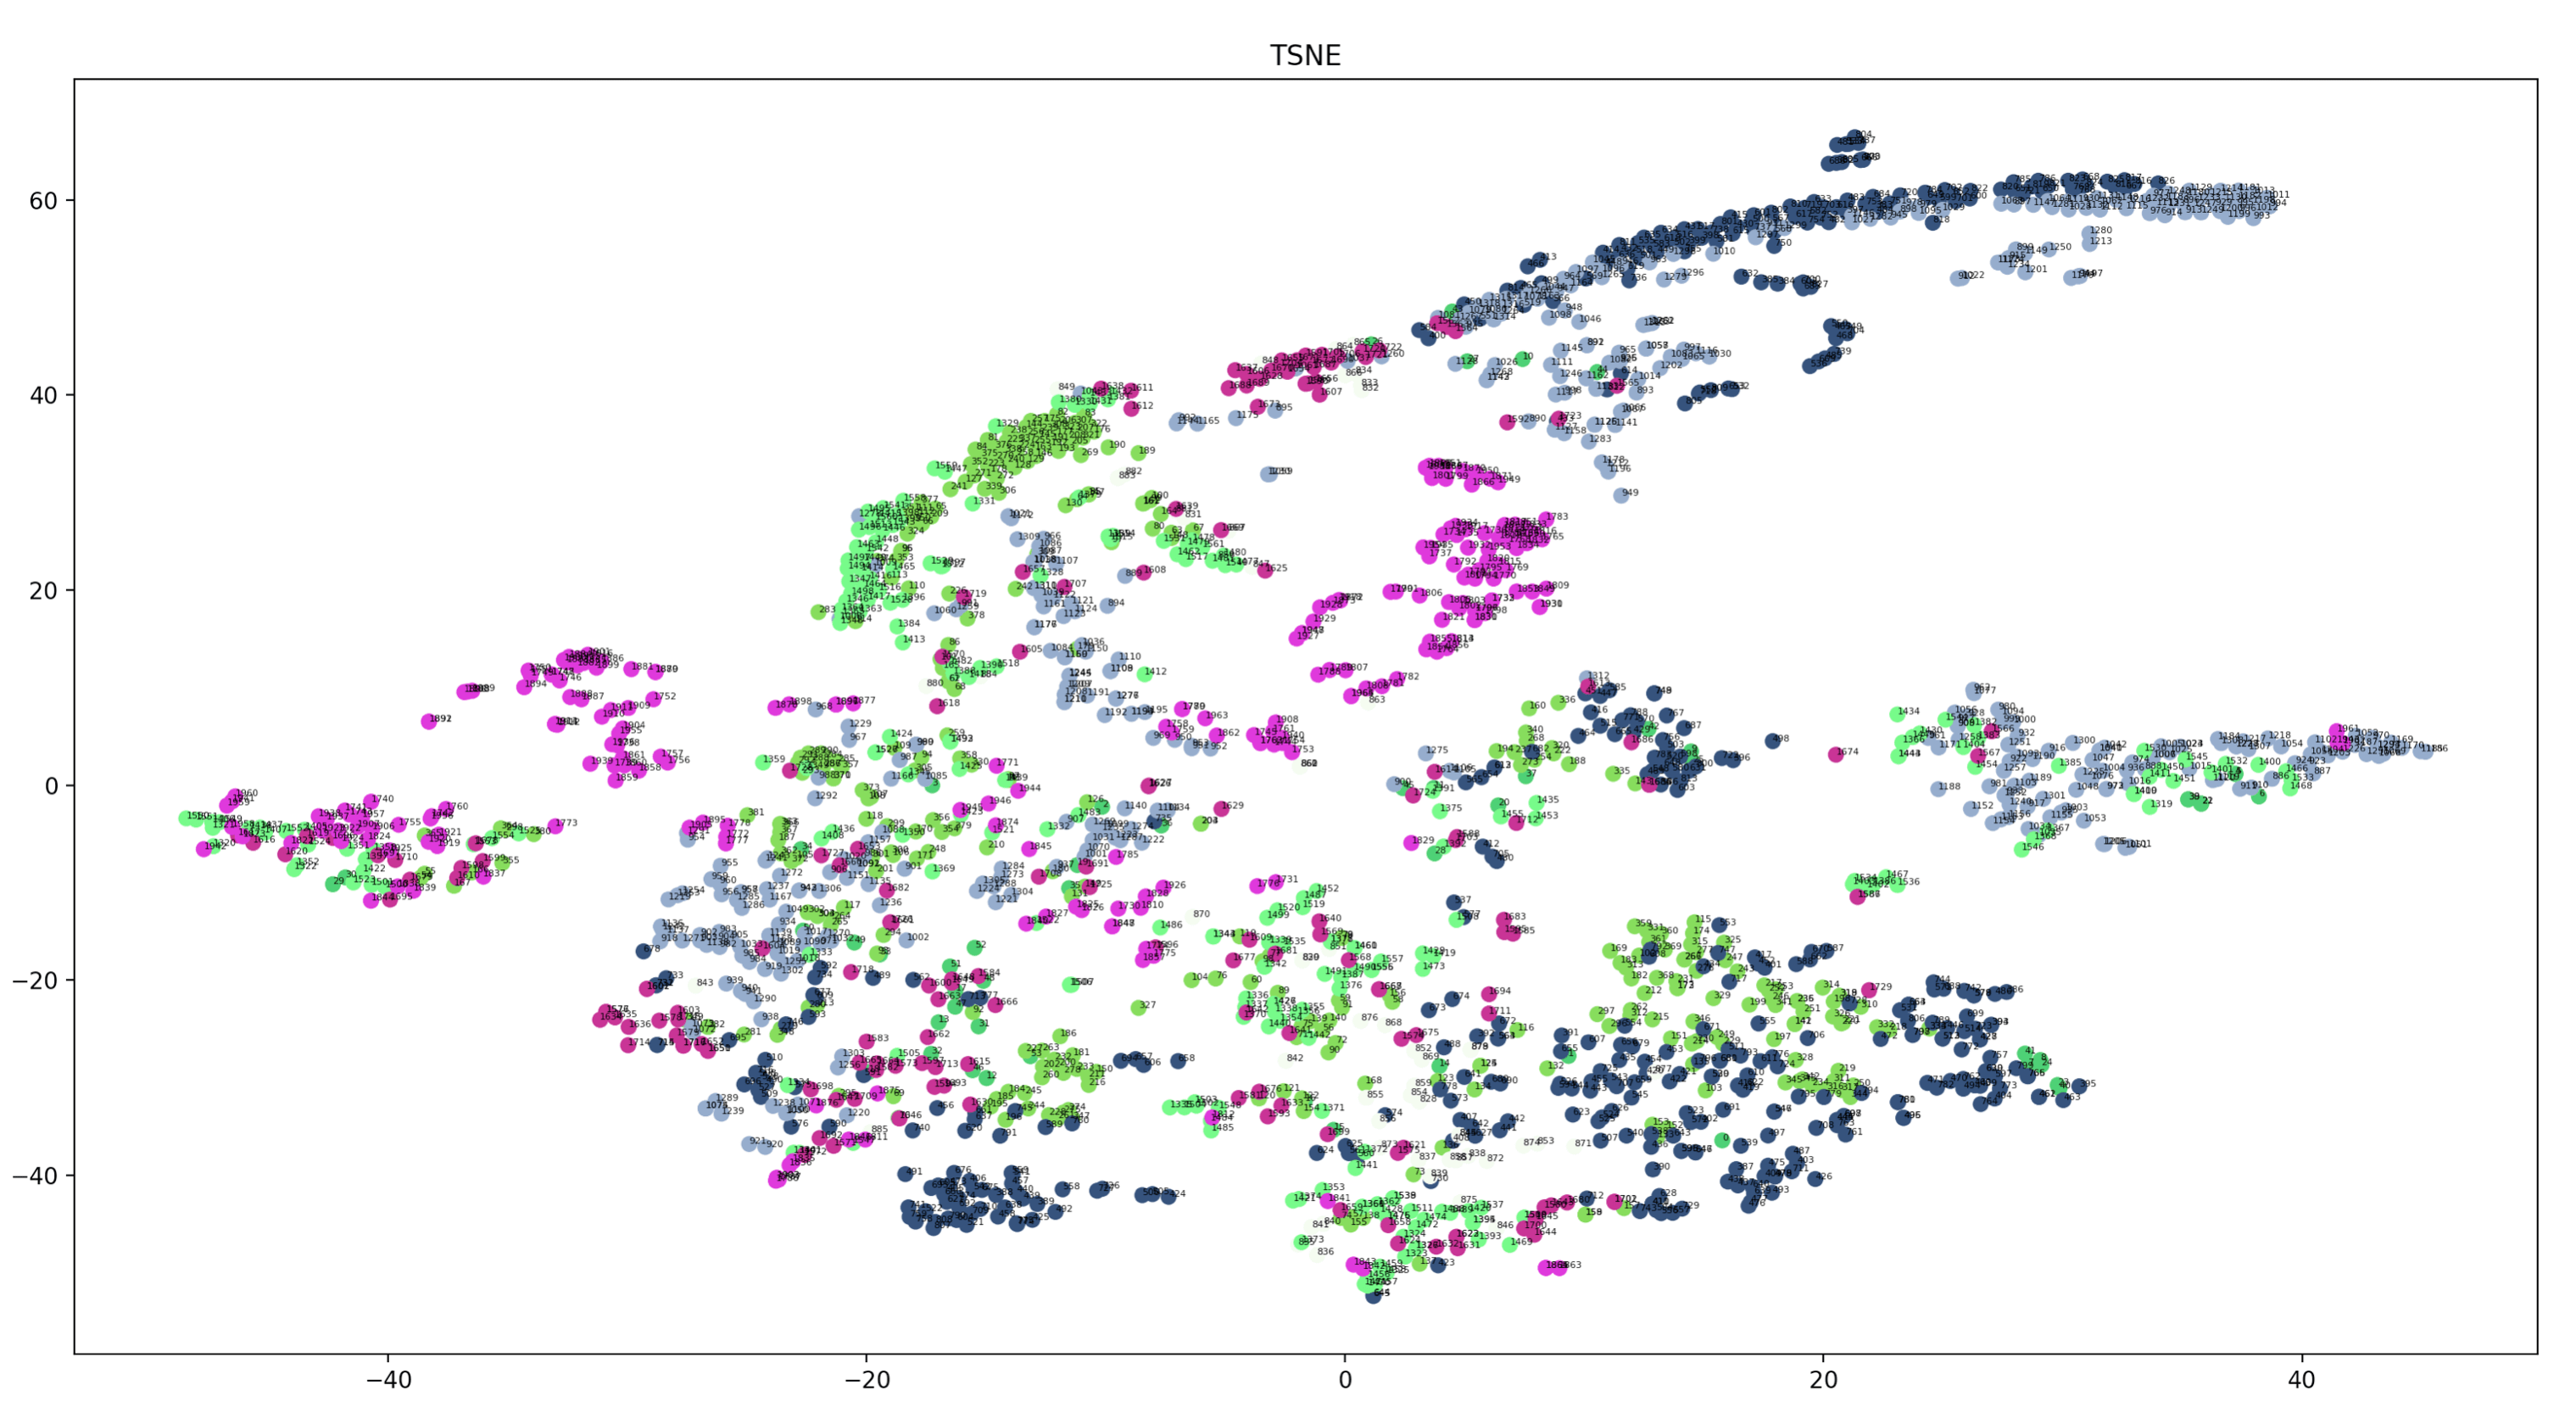
\includegraphics[width=0.9\textwidth]{./images/tsneTestSubjectsColor.png}
  \caption{t-SNE result in a scatter plot, each colour indicates one test subject. The test subjects have clustered together slightly in the chain.}
  \label{figure:tsneTestSubjectsColor}
\end{figure*}

\begin{figure*}[h]
  \centering
  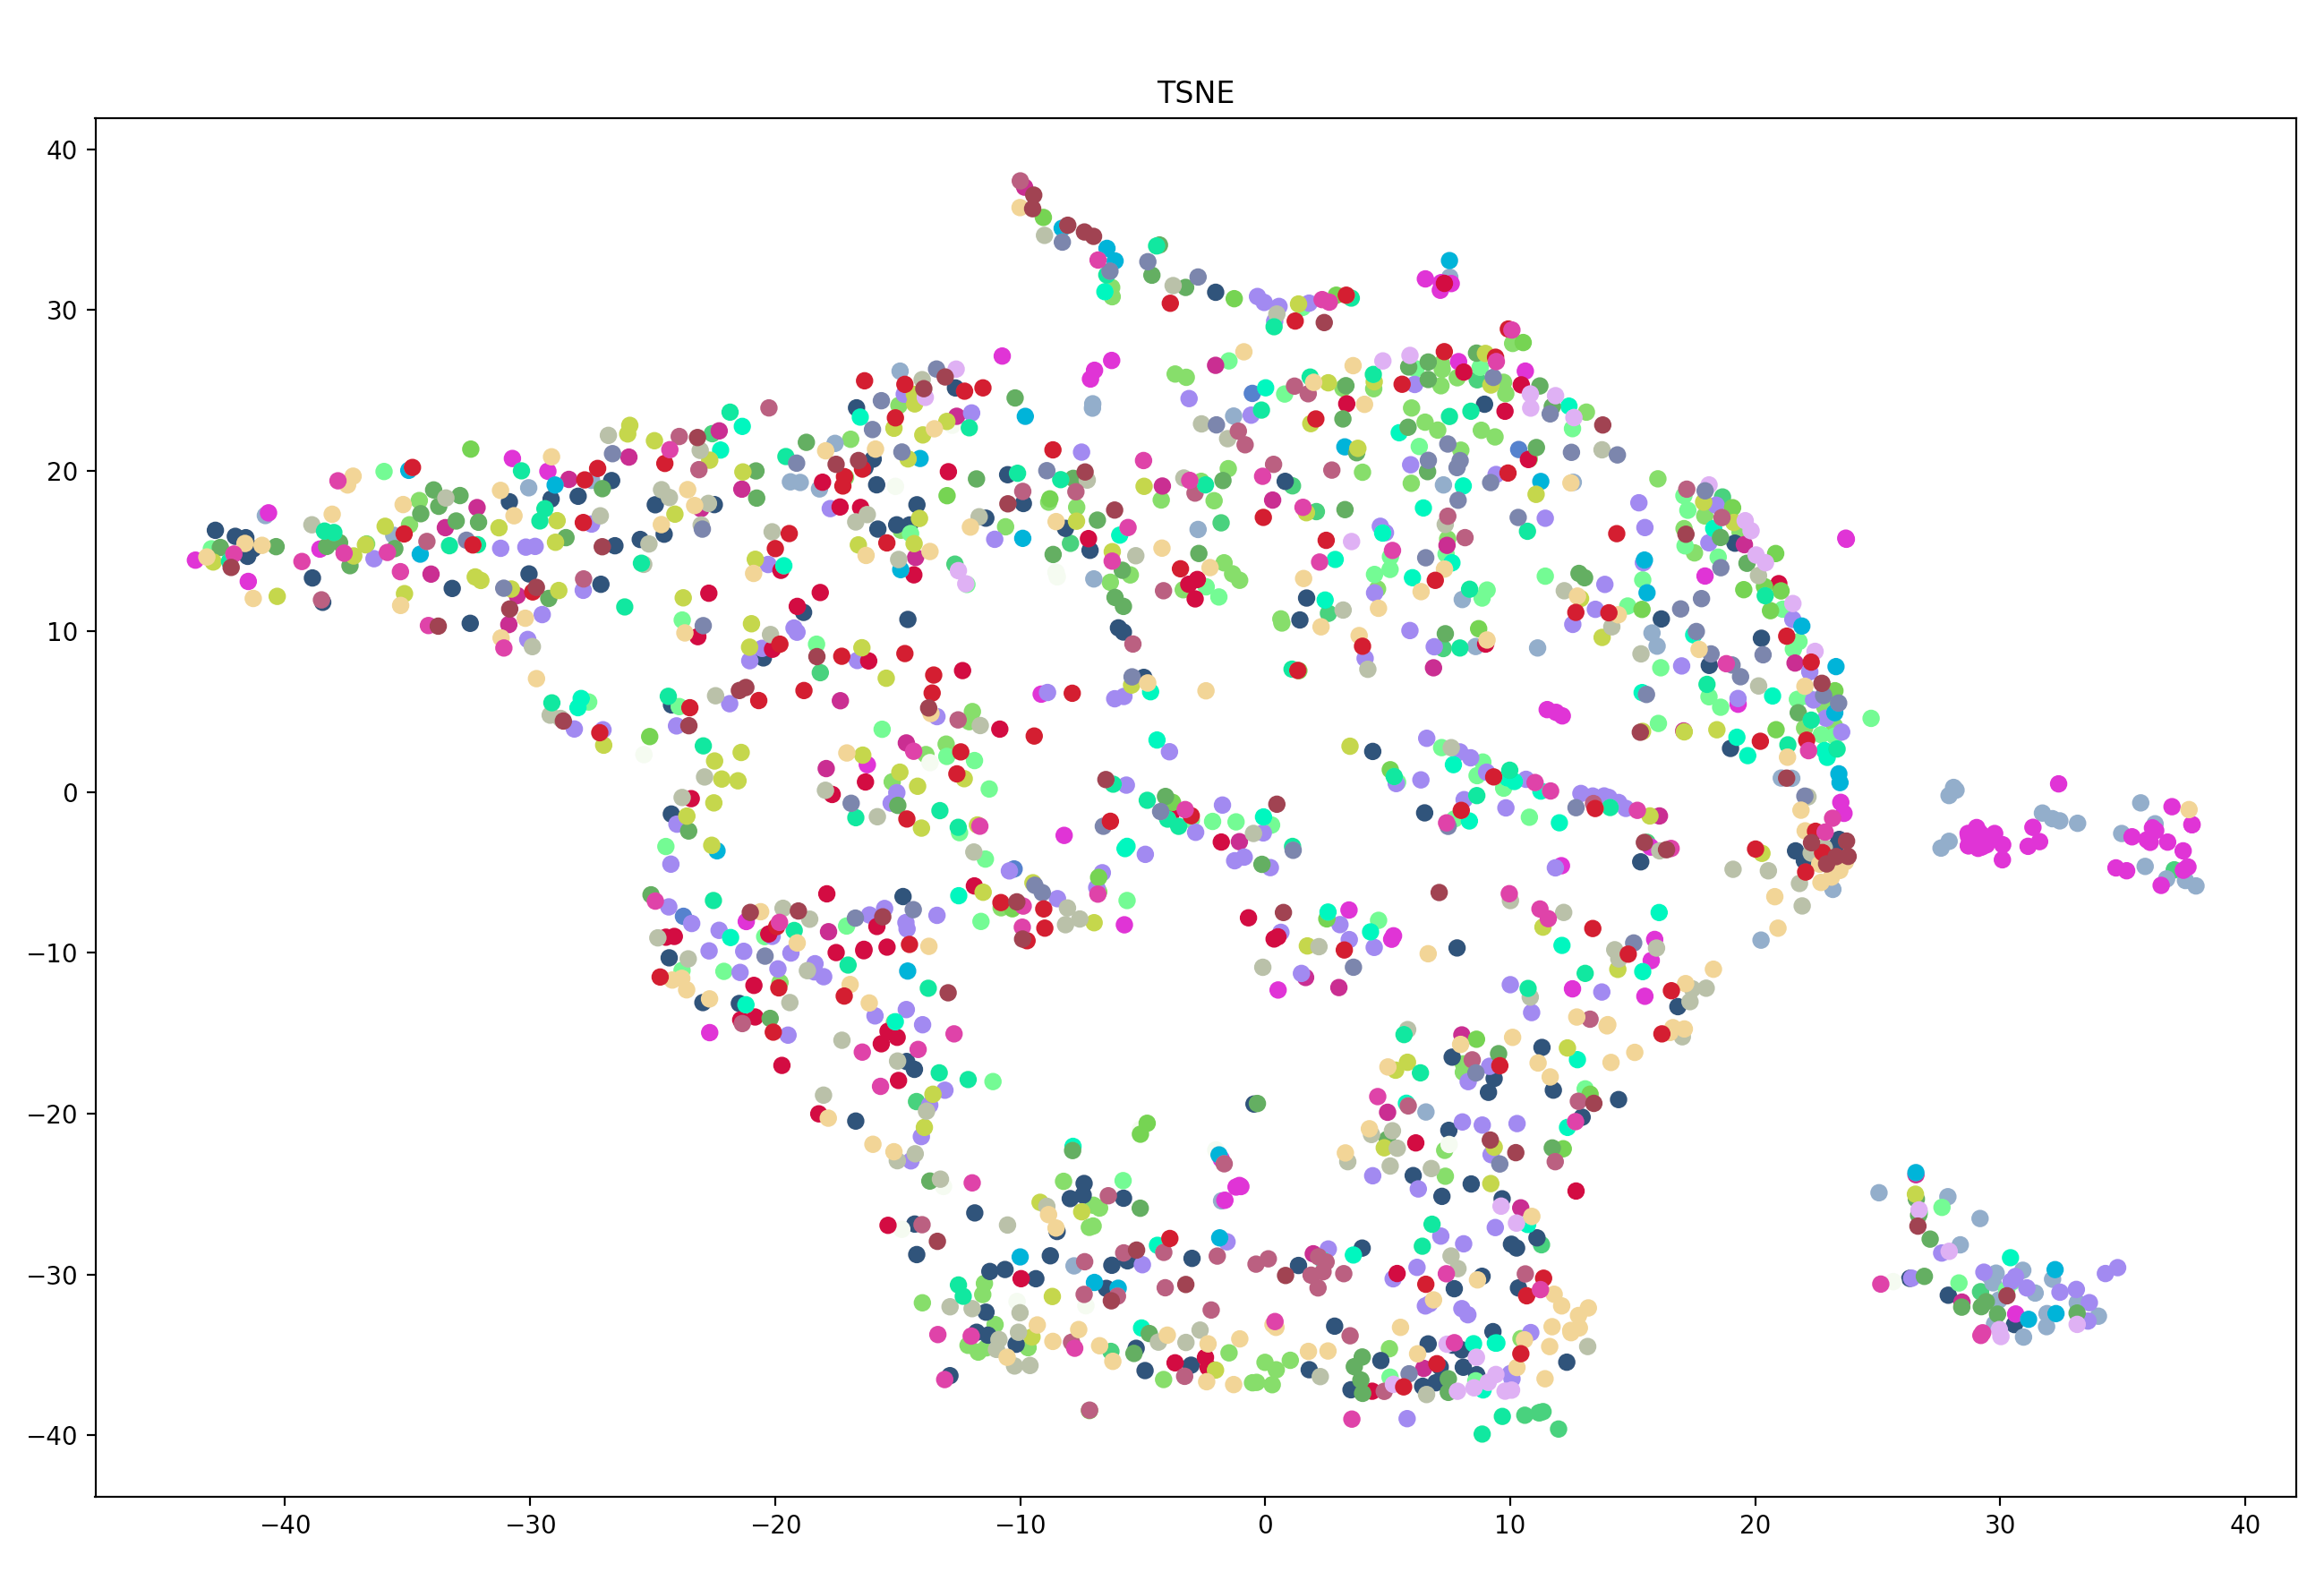
\includegraphics[width=0.9\textwidth]{./images/tsneAfterChainRemoved(50Percent).png}
  \caption{t-SNE calculated after the removal of rows with less than 50\% of values that weren't 0. The chain is less visible and dominant.}
  \label{figure:tsneAfterChainRemoved(50Percent)}
\end{figure*}

% \begin{figure*}[h]
%   \centering
%   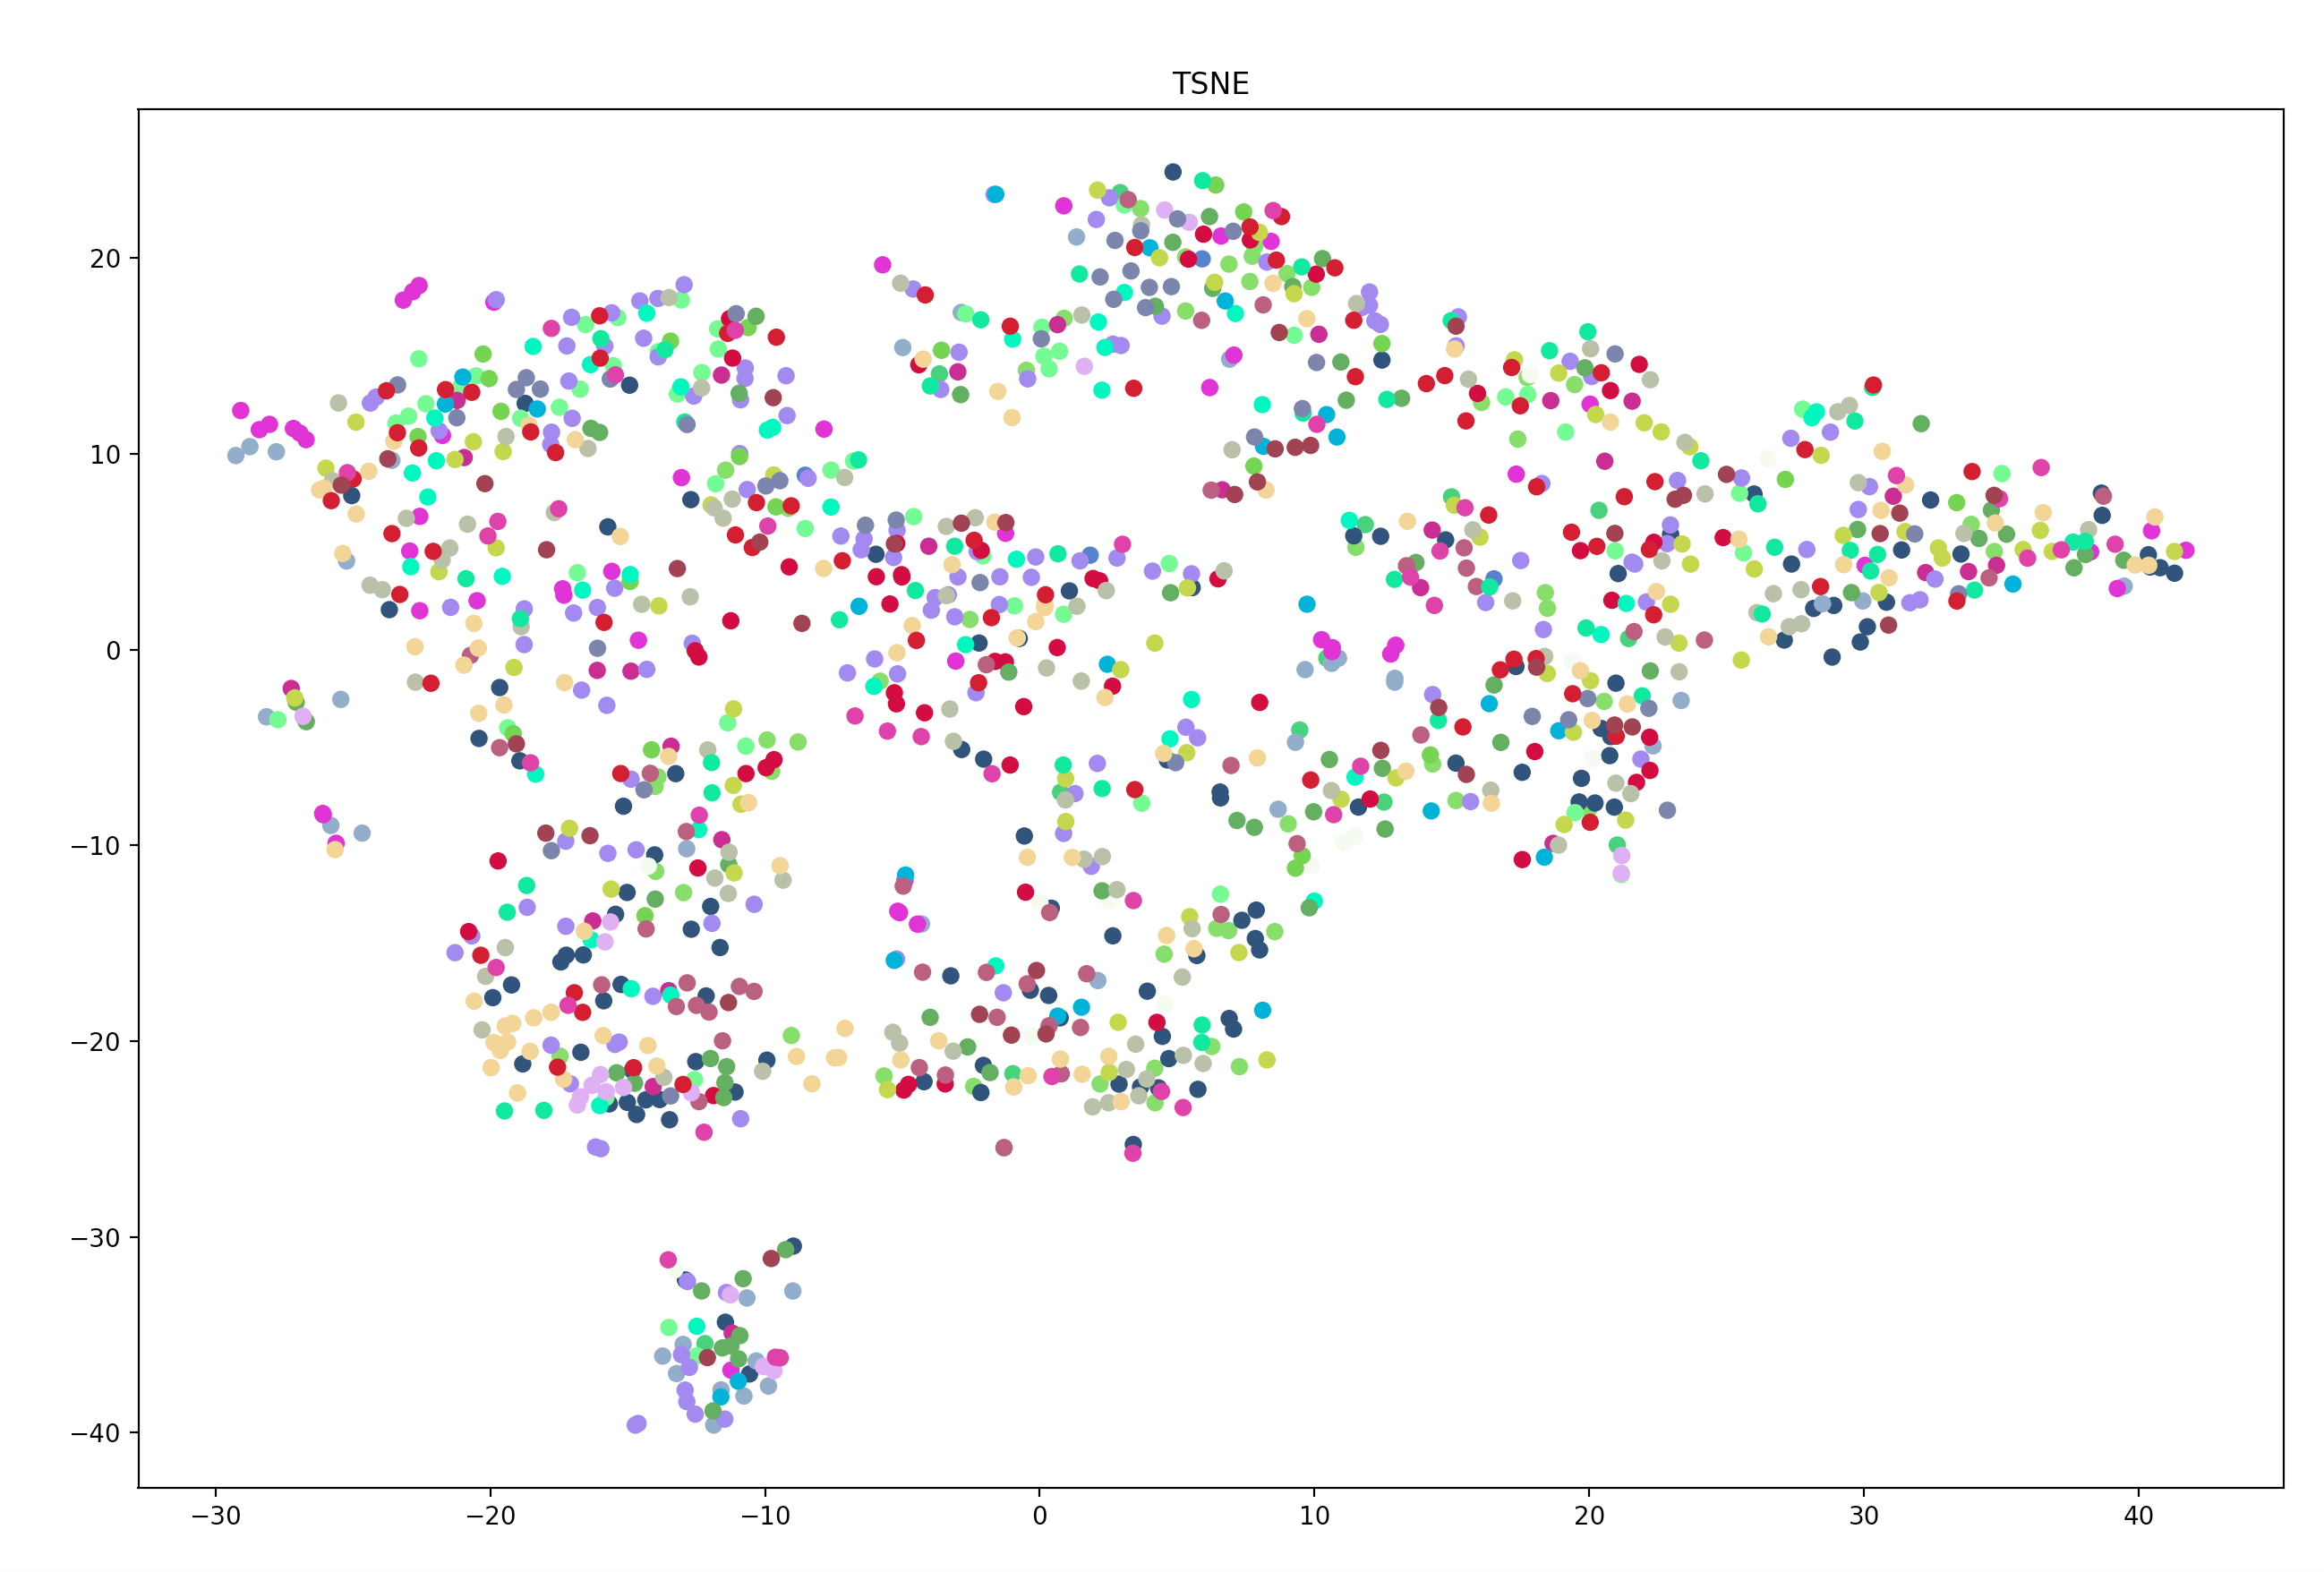
\includegraphics[width=0.9\textwidth]{./images/tsneAfterChainRemoved(60Percent).png}
%   \caption{t-SNE calculated after the removal of rows with less than 60\% of values that weren't 0. The chain is no longer visible.}
%   \label{figure:tsneAfterChainRemoved(60Percent)}
% \end{figure*}

% \begin{figure*}[h]
%   \centering
%   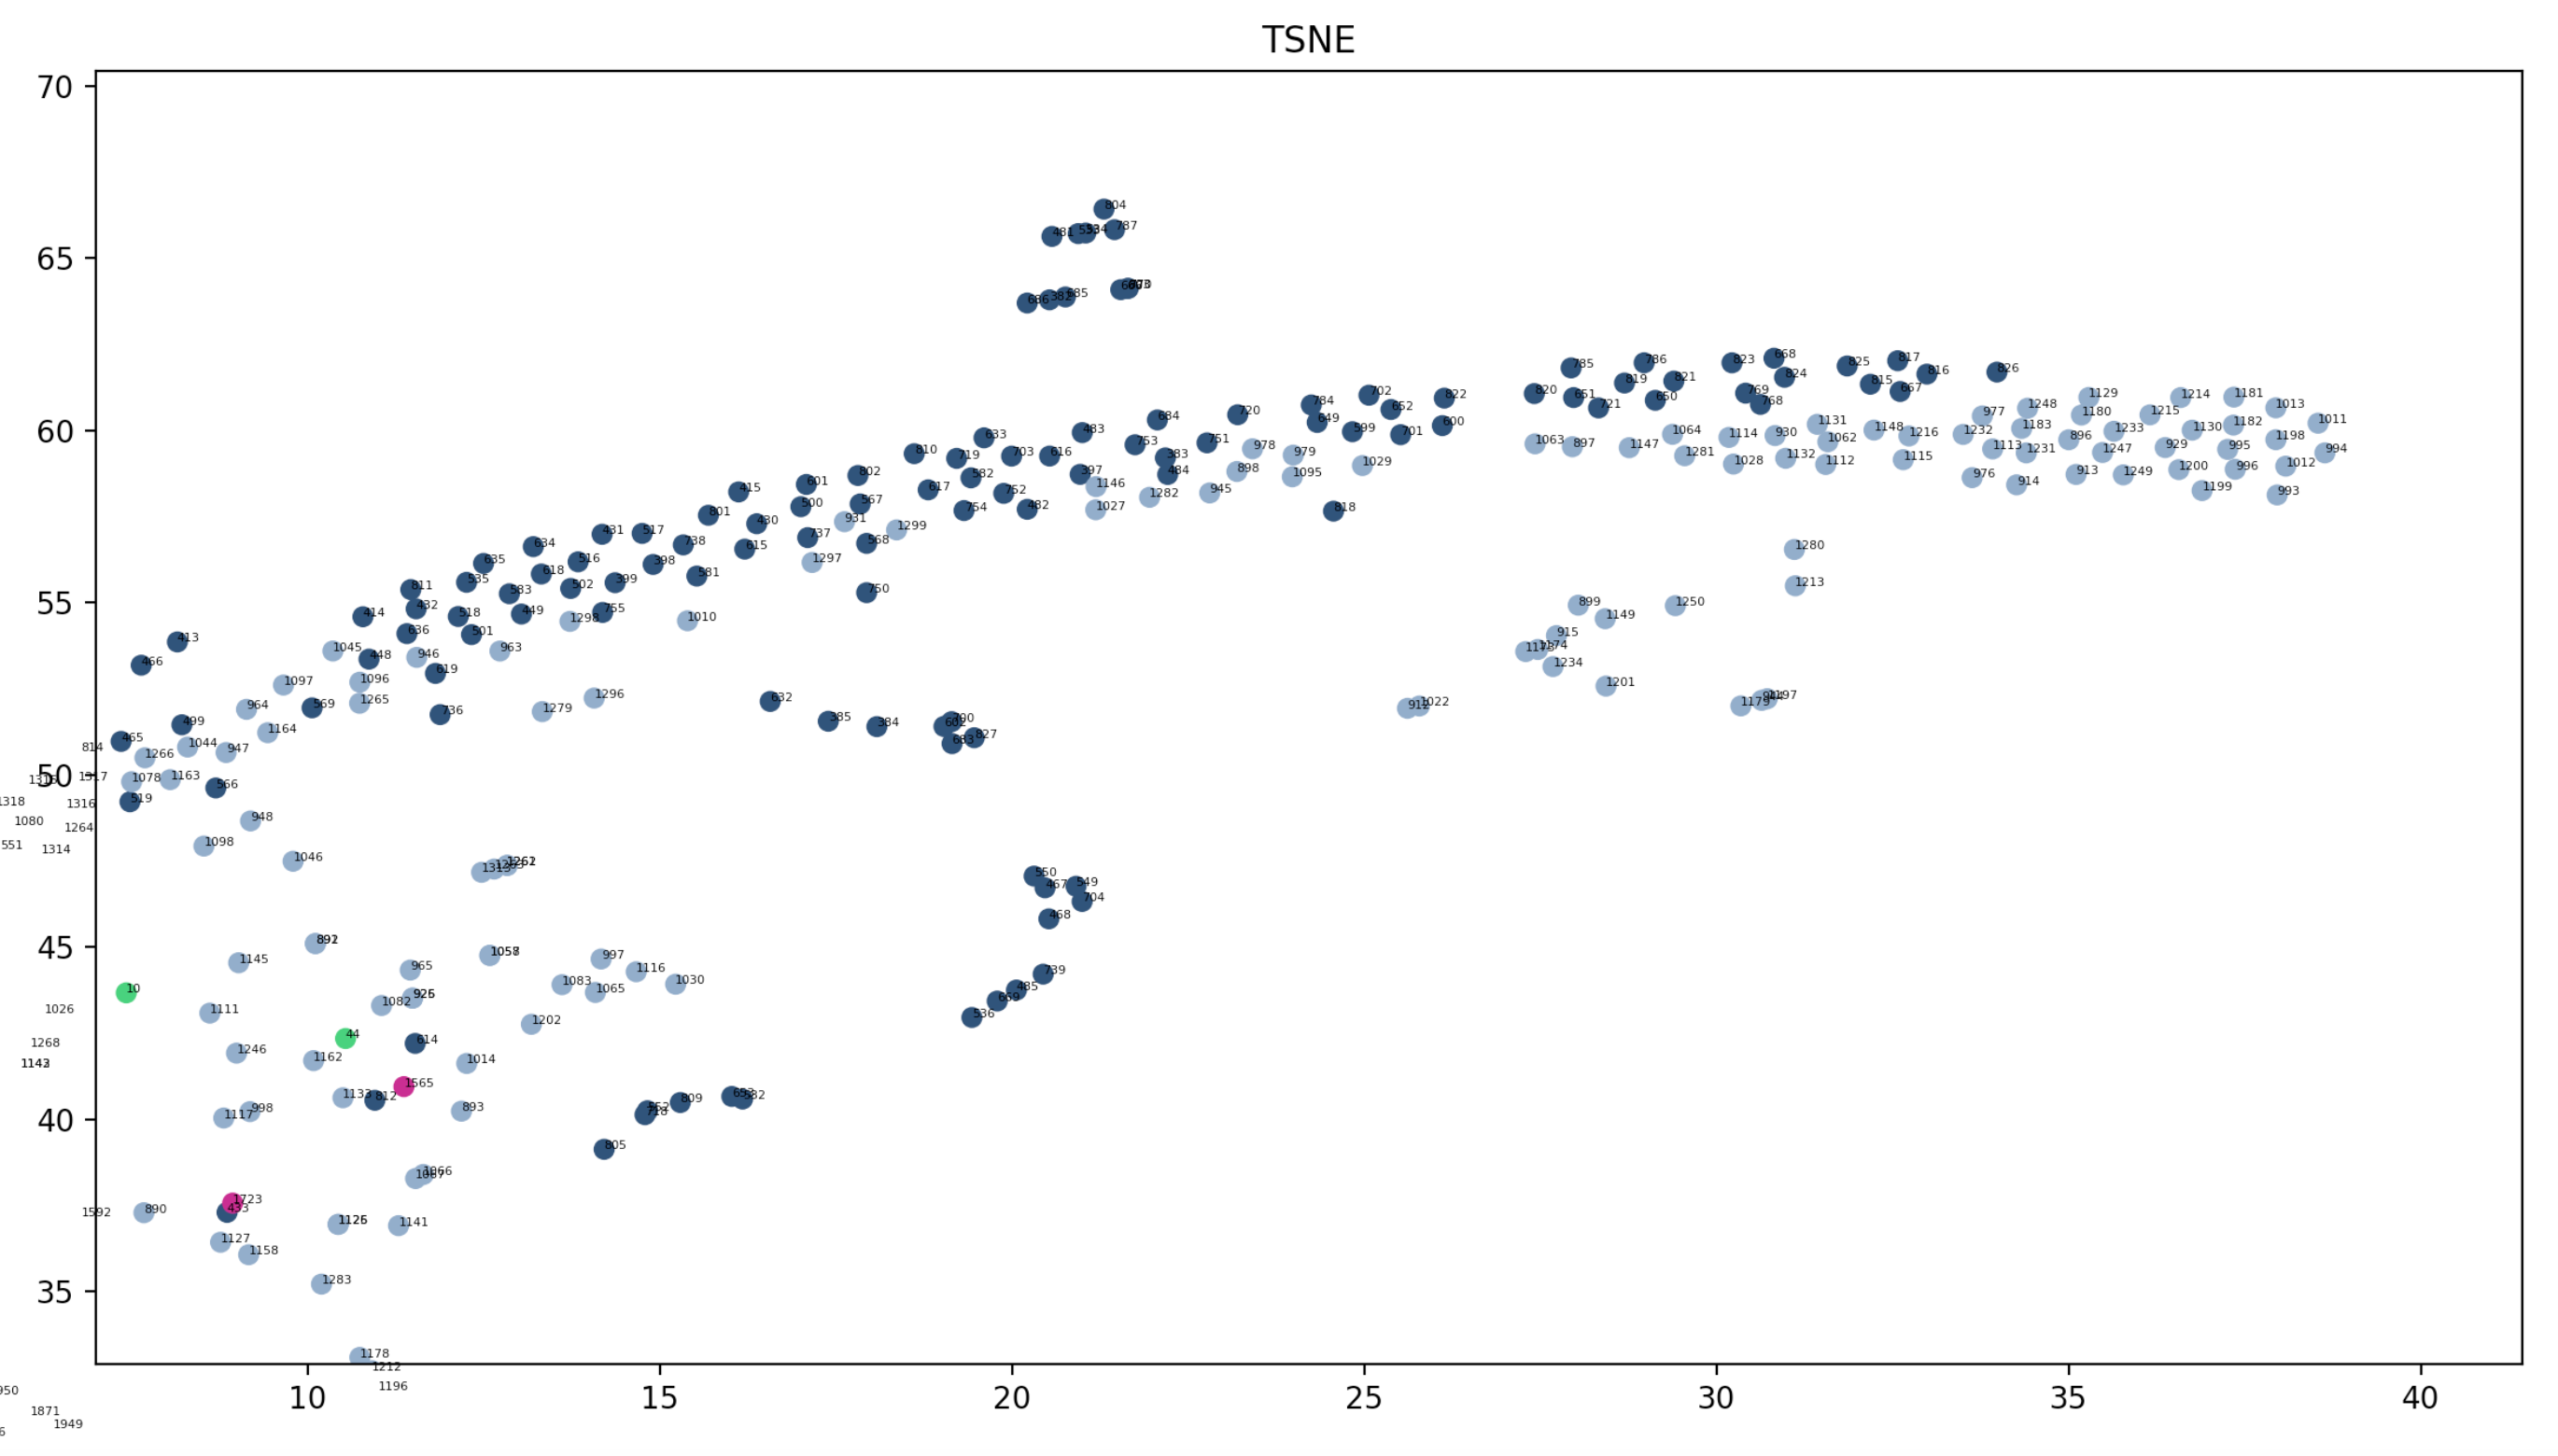
\includegraphics[width=0.9\textwidth]{./images/tsneTestSubjectsColorZoom1.png}
%   \caption{}
%   \label{figure:tsneTestSubjectsColorZoom1}
% \end{figure*}

% \begin{figure*}[h]
%   \centering
%   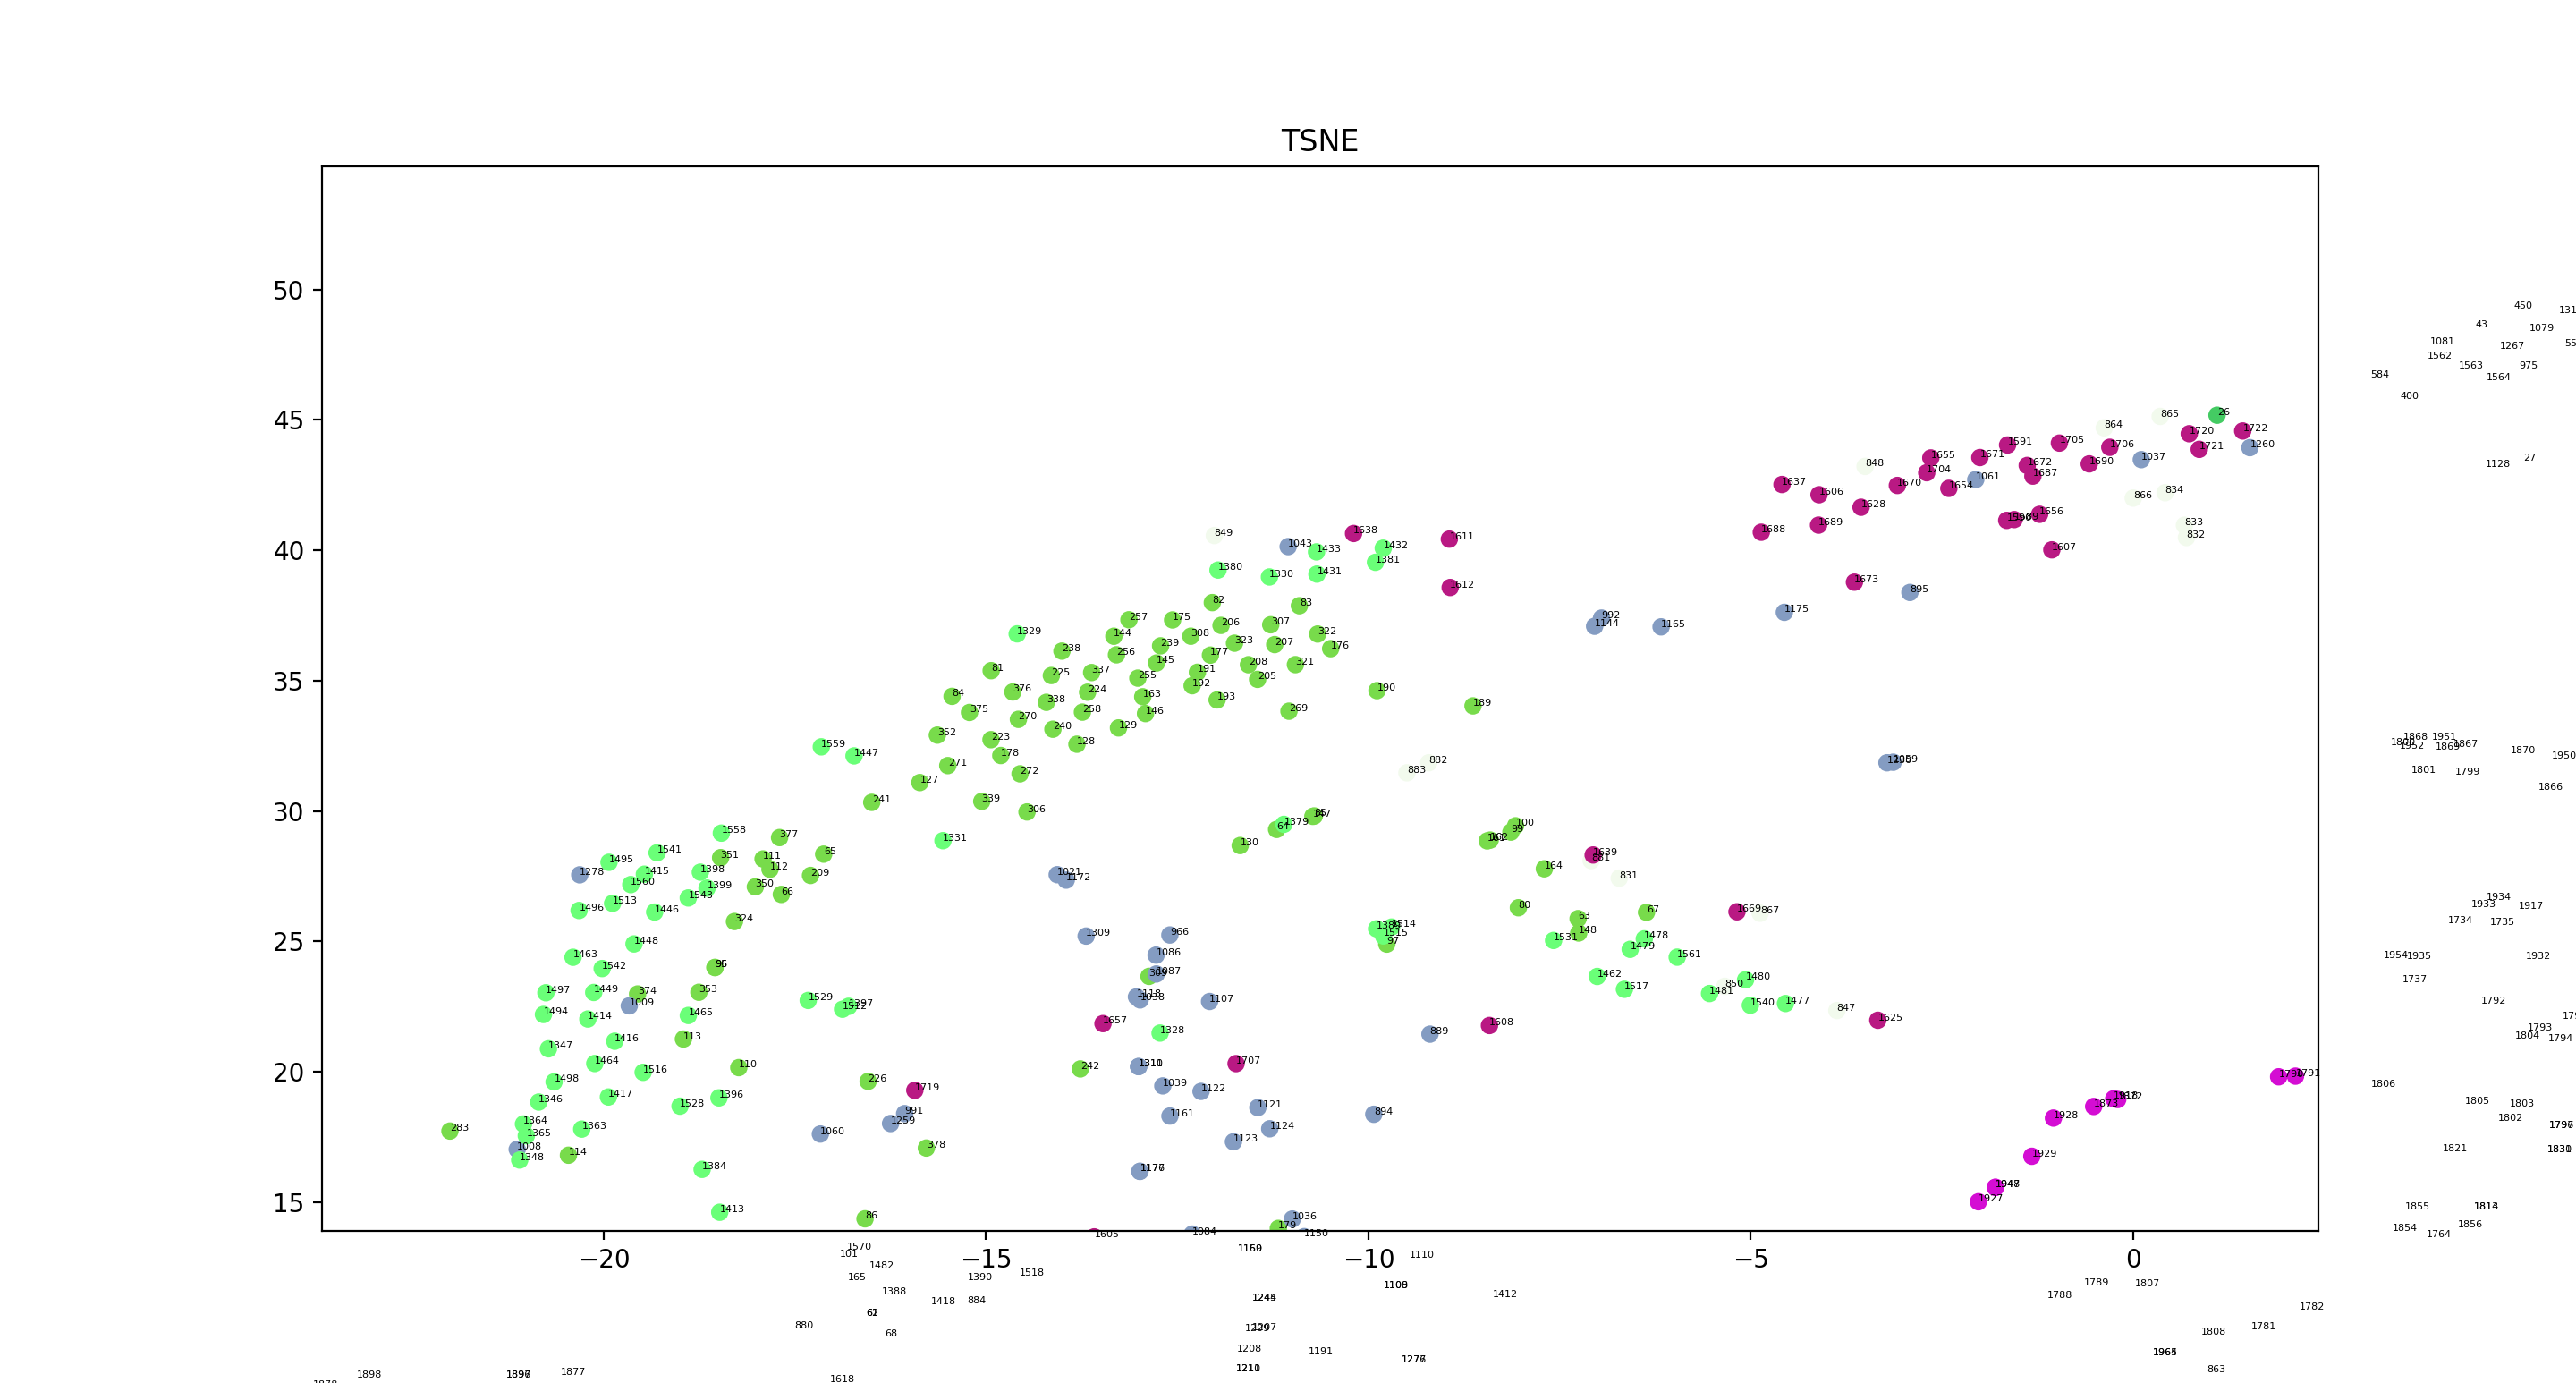
\includegraphics[width=1\textwidth]{./images/tsneTestSubjectsColorZoom2.png}
%   \caption{}
%   \label{figure:tsneTestSubjectsColorZoom2}
% \end{figure*}

% \begin{figure*}[h]
%   \centering
%   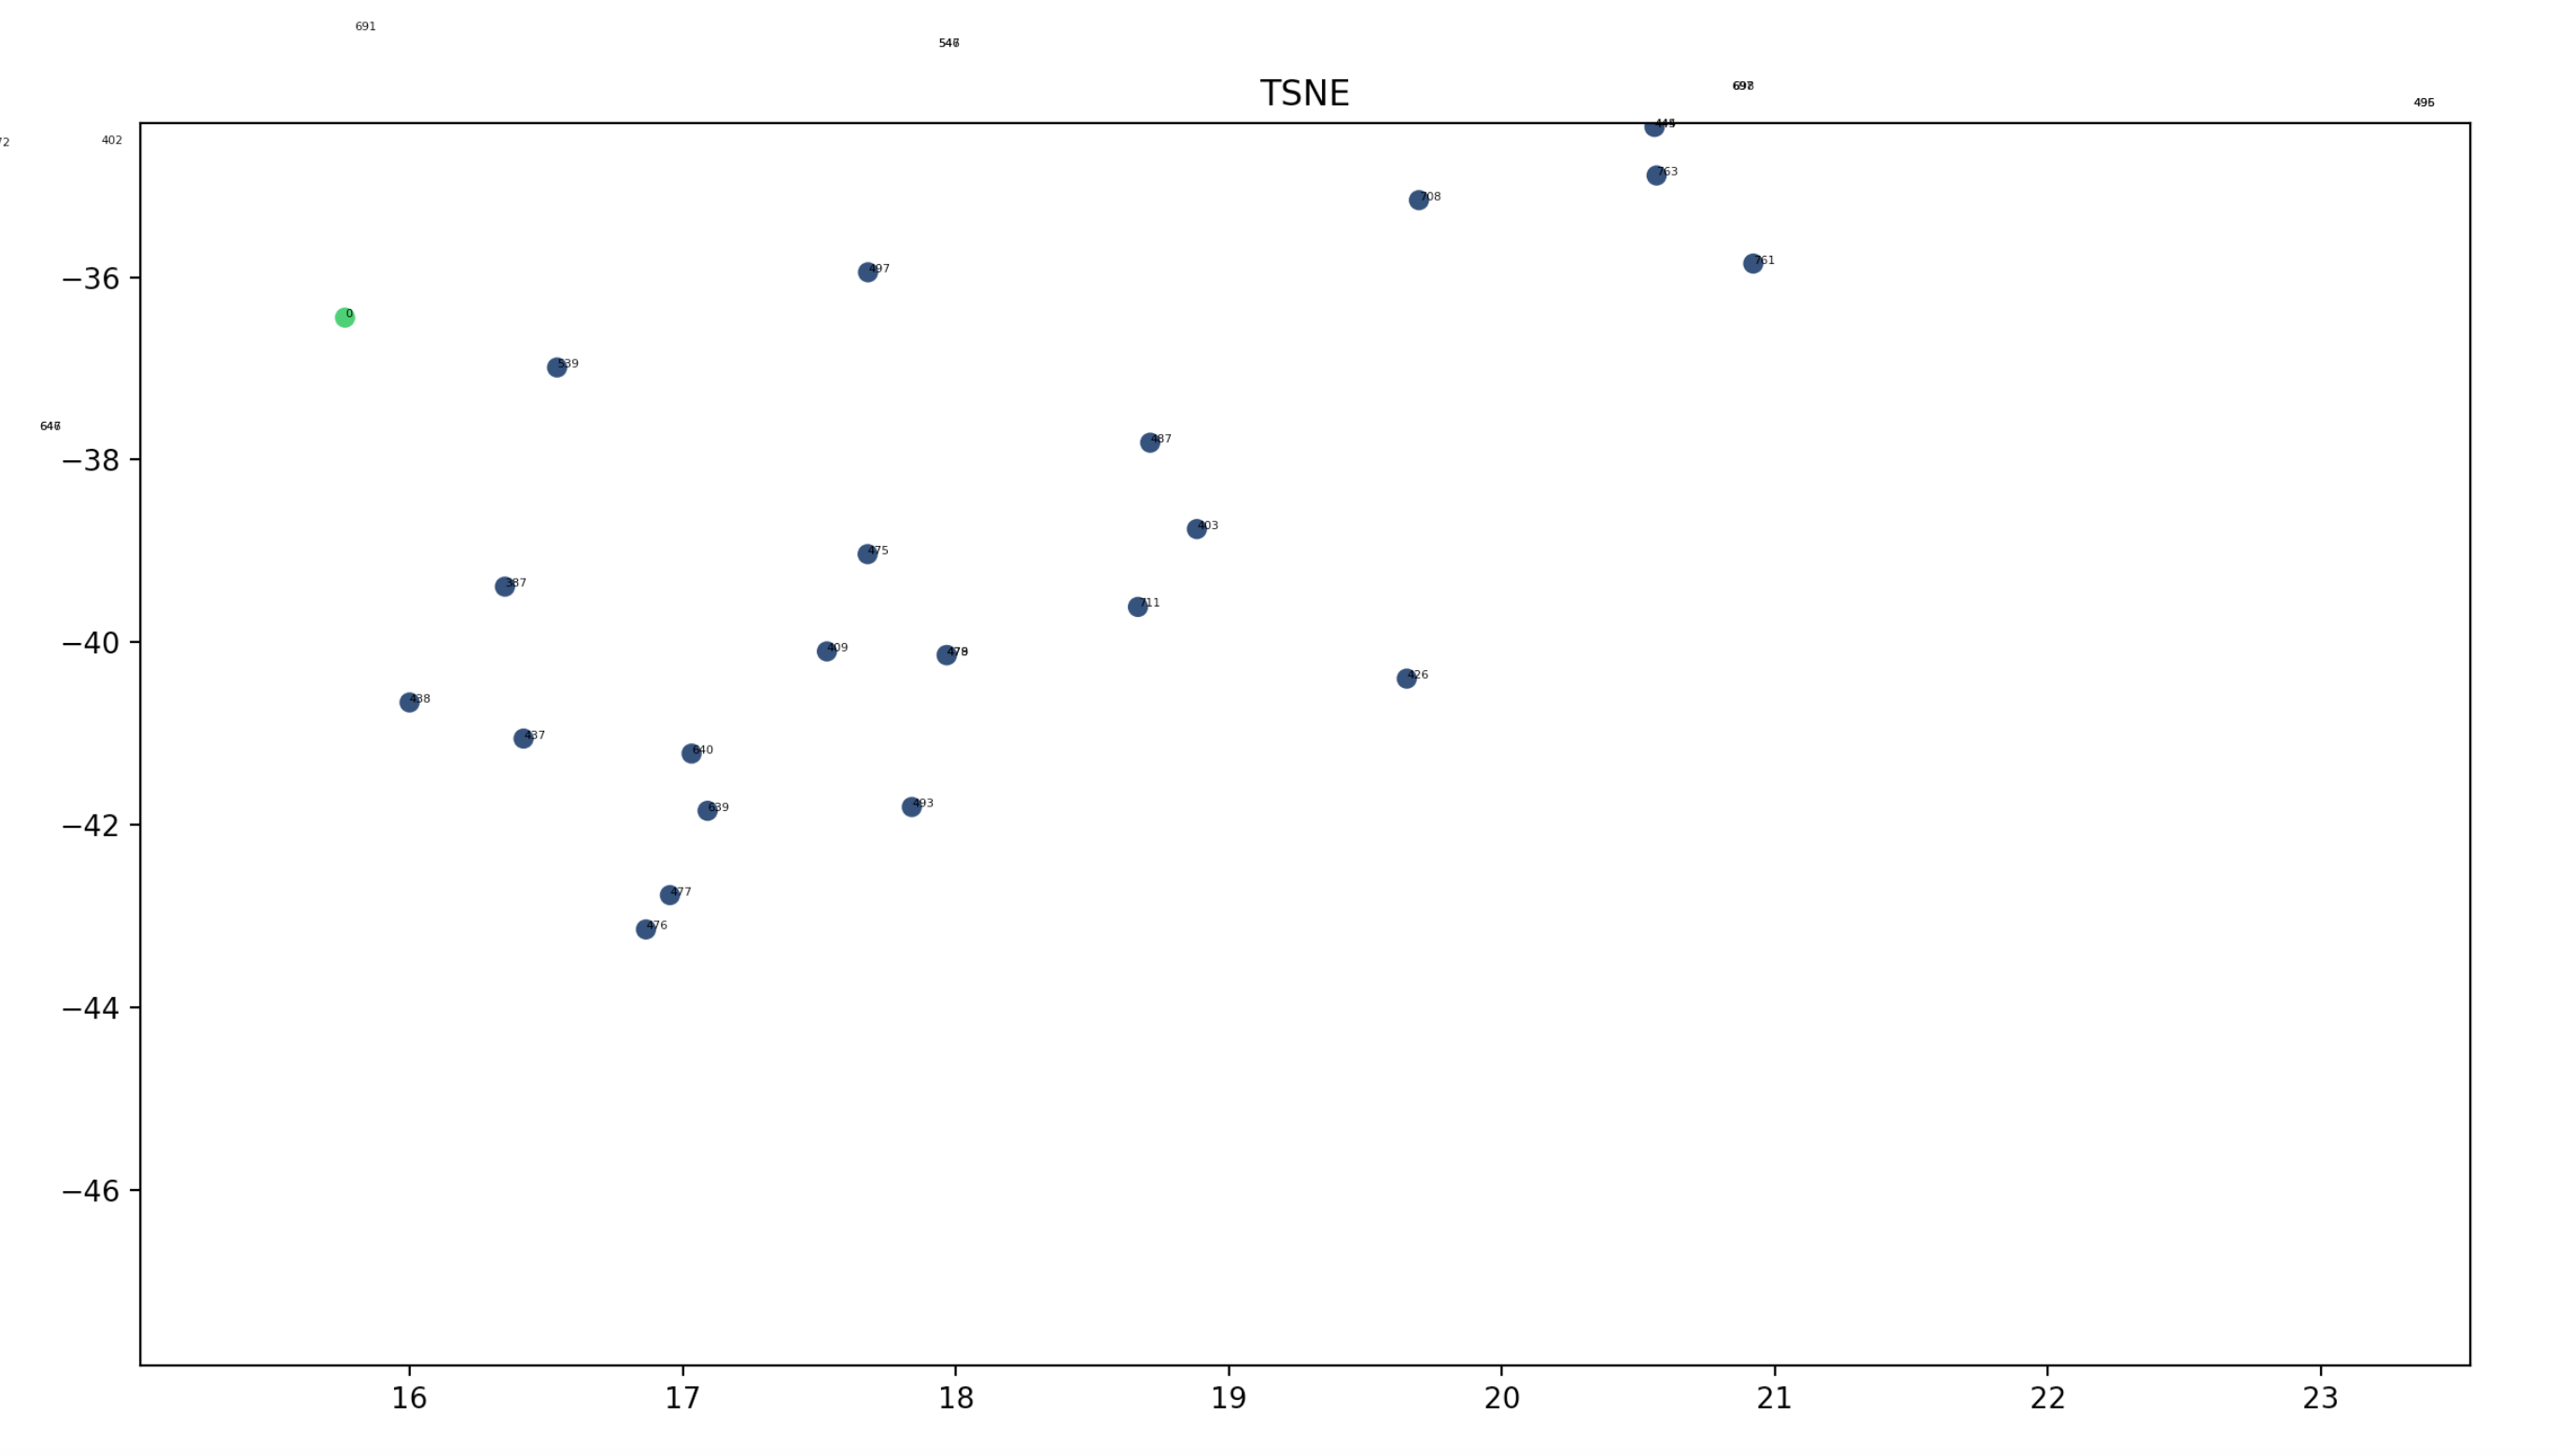
\includegraphics[width=0.9\textwidth]{./images/tsneTestSubjectsColorZoom3.png}
%   \caption{}
%   \label{figure:tsneTestSubjectsColorZoom3}
% \end{figure*}



% Each unique feature only requires one column, and it therefore reduces the number of columns by 

%tod0: say with min max - high value, rest squished together
% \subsubsection{Feature reduction}
% \textbf{todo - finish or remove}
% The deletion of rows with missing values led to the loss of over 50\% of the rows in all time periods. With the intention to preserve as many of these rows as possible, columns with equal to or more than 30\% of rows with missing values were removed. This resulted in only 4 to 5 features of the original 8 being sustained. The results appeared to be unchanged and so, this feature reduction was eventually removed.


% In order to check the functionality of the data preprocessing functions, python tests were written using random mock data.
